%-----------------------------------------------------------------------------%
\chapter{\babLima}
%-----------------------------------------------------------------------------%
\section{Pendahuluan}
Bab ini berisi panduan untuk menggunakan sistem, mencakup panduan bagi pengguna umum (non-teknis) serta panduan instalasi dan konfigurasi bagi pengguna teknis. Selain itu, bab ini juga memuat kesimpulan serta saran untuk pengembangan sistem di masa mendatang.

\section{Panduan Pengguna}

\subsection{Panduan Pengguna Non-Teknis}
\subsubsection{Navigasi Website}

Pada saat pertama kali mengakses website, pengguna akan diarahkan ke halaman \textit{Homepage} yang menampilkan informasi utama terkait kegiatan Lab IR-NLP. Bagian ini mencakup daftar acara mendatang, penjelasan mengenai topik riset yang sedang dikembangkan, serta publikasi terbaru yang dihasilkan oleh anggota lab.

Selain konten utama, pengguna juga dapat menggunakan \textit{navbar} yang tersedia di bagian atas halaman untuk berpindah antar halaman. Menu navigasi tersebut terdiri dari:

\begin{itemize}
    \item \textbf{Peoples}: berisi daftar anggota lab yang dikelompokkan menjadi \textit{Faculty Members}, \textit{Current Students}, dan \textit{Alumni}.
    
    \item \textbf{Publications}: menampilkan daftar publikasi ilmiah yang dihasilkan oleh anggota lab, termasuk detail penulis, topik, dan tautan ke sumber asli.

    \item \textbf{Research Grants}: menyajikan informasi mengenai hibah penelitian (\textit{research grants}) yang pernah diterima atau sedang dikerjakan oleh lab.

    \item \textbf{Tools \& Resources}: menampilkan koleksi perangkat lunak (software tools) dan dataset yang dikembangkan oleh Lab IR-NLP.

    \item \textbf{Events}: menampilkan seluruh kegiatan akademik seperti seminar, lokakarya, dan \textit{talk series} yang diselenggarakan oleh lab.

    \item \textbf{Contact}: berisi informasi kontak resmi Lab IR-NLP yang dapat digunakan untuk keperluan komunikasi atau kerja sama.
\end{itemize}

Website juga dilengkapi dengan fitur pemilihan bahasa melalui menu \textit{language dropdown} yang memungkinkan pengguna mengganti bahasa tampilan antara Bahasa Indonesia dan Bahasa Inggris.

\subsubsection{Mengakses Informasi Publikasi}
Halaman publikasi dapat diakses melalui menu \textit{Publications} pada navbar. Pada halaman ini, publikasi ditampilkan berdasarkan tahun terbit dan diurutkan dari yang paling baru. Pengguna juga dapat melakukan pencarian menggunakan \textit{search bar} untuk menemukan publikasi tertentu. Selain itu, pengguna dapat membuka halaman detail publikasi atau menuju tautan DOI dengan menekan judul publikasi yang tersedia.

\subsubsection{Melihat Daftar Hibah Penelitian}
Halaman ini dapat diakses melalui menu \textit{Research} pada navbar. Pada halaman ini, pengguna dapat melihat informasi mengenai hibah penelitian yang telah diperoleh oleh Lab IR-NLP, termasuk nama hibah, penyedia hibah, serta periode pelaksanaannya.

\subsubsection{Melihat Daftar Anggota (People)}
Halaman \textit{People} dapat diakses melalui navbar dan menampilkan daftar anggota Lab IR-NLP yang dikelompokkan ke dalam tiga kategori utama:
\begin{itemize}
    \item \textbf{Faculty Members}: berisi daftar dosen yang tergabung dalam Lab IR-NLP.
    \item \textbf{Current Students}: menampilkan mahasiswa yang saat ini dibimbing oleh lab, beserta topik penelitian yang relevan dengan bidang kajian IR dan NLP.
    \item \textbf{Alumni}: menampilkan daftar mahasiswa yang telah menyelesaikan studi dan menjadi alumni Lab IR-NLP.
\end{itemize}
Setiap kategori disajikan dalam tampilan terstruktur sehingga pengguna dapat dengan mudah menelusuri profil anggota lab.

\subsubsection{Mengakses Halaman Event}
Halaman \textit{Events} dapat diakses melalui menu navigasi utama. Pada halaman ini, daftar kegiatan akademik yang diselenggarakan oleh Lab IR-NLP ditampilkan dalam dua kategori utama, yaitu:
\begin{itemize}
    \item \textbf{IR-NLP Talks}: berisi rangkaian sesi diskusi atau presentasi yang membahas topik-topik terkait Information Retrieval dan Natural Language Processing.
    \item \textbf{Seminar}: menampilkan berbagai seminar akademik yang diselenggarakan secara internal maupun eksternal.
\end{itemize}
Setiap acara ditampilkan dengan informasi utama seperti judul, deskripsi singkat, tanggal pelaksanaan, serta tautan pertemuan (jika tersedia).

\subsubsection{Menggunakan Resource dan Tools}
Halaman \textit{Tools \& Resources} menampilkan berbagai perangkat lunak (software tools) serta dataset yang dikembangkan oleh Lab IR-NLP. Pada halaman ini, pengguna dapat melihat daftar alat pemrosesan bahasa alami maupun himpunan data yang telah dihasilkan dalam kegiatan penelitian laboratorium. Setiap item dilengkapi dengan deskripsi singkat dan tautan terkait jika tersedia.

\subsubsection{Menggunakan Halaman Kontak}
Halaman \textit{Contact} menyediakan informasi resmi mengenai cara menghubungi Lab IR-NLP, termasuk alamat email, lokasi laboratorium, serta tautan terkait lainnya. Melalui halaman ini, pengguna dapat memperoleh informasi kontak yang diperlukan atau mengirimkan pesan melalui formulir yang telah disediakan (jika tersedia).

\subsection{Panduan Pengguna Teknis}
\subsubsection{Kebutuhan Sistem}
Untuk menjalankan sistem, pengguna dapat memilih dua metode, yaitu menggunakan \textit{Docker container} atau melakukan instalasi langsung pada lingkungan lokal. Sistem ini memerlukan lingkungan berbasis Linux atau WSL karena aplikasi memanfaatkan paket \texttt{django-cron} yang hanya dapat berjalan pada sistem operasi Linux.

Selain itu, sistem membutuhkan Python versi 3.10 atau lebih baru, serta \textit{package dependencies} lain yang telah dicantumkan secara lengkap pada berkas \texttt{requirements.txt}. Penggunaan \textit{virtual environment} direkomendasikan untuk memastikan isolasi paket dan stabilitas lingkungan pengembangan.

\subsubsection{Instalasi Aplikasi}
Instalasi aplikasi dapat dilakukan melalui dua metode, yaitu instalasi manual menggunakan Python atau menggunakan Docker.

\paragraph{1. Instalasi Manual}
Berikut langkah-langkah instalasi aplikasi secara manual:

\begin{enumerate}
    \item \textbf{Membuat dan mengaktifkan \textit{virtual environment}}  
    Membuat \textit{virtual environment} dengan perintah:  
    \begin{verbatim}
    python -m venv venv
    \end{verbatim}
    Kemudian mengaktifkannya menggunakan:  
    \begin{verbatim}
    source venv/bin/activate
    \end{verbatim}

    \item \textbf{Menginstal seluruh dependensi aplikasi}  
    Seluruh dependensi dapat dipasang melalui berkas \texttt{requirements.txt} dengan perintah:  
    \begin{verbatim}
    pip install -r requirements.txt
    \end{verbatim}

    \item \textbf{Melakukan migrasi database}  
    Perintah berikut digunakan untuk membuat struktur tabel sesuai model:  
    \begin{verbatim}
    python manage.py migrate
    \end{verbatim}

    \item \textbf{Menjalankan server pengembangan}  
    Untuk menjalankan aplikasi, gunakan:  
    \begin{verbatim}
    python manage.py runserver
    \end{verbatim}
\end{enumerate}

\paragraph{2. Instalasi Menggunakan Docker}
Selain instalasi manual, aplikasi juga dapat dijalankan menggunakan Docker. Instalasi dapat dilakukan melalui satu perintah berikut:

\begin{verbatim}
docker compose up --build -d
\end{verbatim}

Perintah tersebut secara otomatis membangun image, menjalankan container, dan mengonfigurasi lingkungan aplikasi.

\subsubsection{Struktur Proyek}
Penjelasan direktori:

\begin{itemize}
    \item \texttt{templates/} \\
    Direktori ini digunakan untuk menyimpan seluruh template aplikasi, yaitu file HTML yang bersifat statis dan digunakan secara global di seluruh aplikasi. Contohnya meliputi \textit{base.html}, halaman utama, \textit{navbar}, dan \textit{sidebar}.

    \item \texttt{static/} \\
    Direktori ini digunakan untuk menyimpan seluruh aset statis aplikasi Django seperti file CSS, JavaScript, gambar, dan aset pendukung lainnya yang digunakan dalam tampilan antarmuka aplikasi.

    \item \texttt{lab\_ir\_nlp\_settings/} \\
    Direktori ini merupakan folder utama proyek yang berisi konfigurasi global aplikasi, termasuk pengaturan aplikasi, konfigurasi deployment, koneksi database, dan konfigurasi lain yang bersifat menyeluruh.

    \item \texttt{core/} \\
    Direktori ini merupakan aplikasi utama yang digunakan untuk menjalankan \textit{views} halaman utama serta menjadi tempat penyimpanan model-model utama dari aplikasi.

    \item \texttt{events/} \\
    Direktori ini merupakan aplikasi yang digunakan untuk mengelola fitur \textit{events}, termasuk penyimpanan konfigurasi, \textit{views}, dan \textit{URL routing} yang berkaitan dengan halaman \textit{events} beserta tampilan HTML dan CSS-nya.

    \item \texttt{publications/} \\
    Direktori ini merupakan aplikasi yang digunakan untuk mengelola publikasi dan \textit{research grants}. Folder ini mencakup proses \textit{scraping} data publikasi, halaman tampilan (HTML dan CSS), konfigurasi aplikasi, serta pembuatan dan pengelolaan model dan integrasi \textit{Google Sheets} \textit{research grant}.
    
    \item \texttt{tools/} \\
    Direktori ini merupakan aplikasi yang digunakan untuk menyimpan dan mengelola \textit{views} serta \textit{URL routing} dari berbagai fitur \textit{tools} dan dataset yang digunakan dalam aplikasi.
    
    \item \texttt{media/} \\
    Direktori ini digunakan untuk menyimpan file yang diunggah melalui halaman admin (misalnya dokumen, gambar, atau file pendukung lainnya).
    
    \item \texttt{locale/} \\
    Direktori ini digunakan untuk menyimpan konfigurasi serta file \texttt{.po} dan \texttt{.mo} yang berisi hasil penerjemahan (\textit{translation}) aplikasi, sehingga mendukung penggunaan dua bahasa, yaitu Bahasa Indonesia dan Bahasa Inggris.
\end{itemize}

\subsubsection{Menjalankan Server Django}
Panduan menjalankan server lokal melalui \texttt{python manage.py runserver}.

\subsubsection{Penggunaan Halaman Admin Django}

Aplikasi ini menggunakan fitur bawaan dari Django Admin untuk melakukan pengelolaan data secara terpusat melalui antarmuka berbasis web. Halaman admin hanya dapat diakses oleh pengguna yang memiliki hak akses (administrator atau staf) dan digunakan untuk mengelola berbagai data penting dalam sistem.

\textbf{Cara login ke halaman admin:}
\begin{enumerate}
    \item Jalankan server Django menggunakan perintah \texttt{python manage.py runserver}.
    \item Buka browser dan akses alamat berikut: \texttt{http://localhost:8000/admin/}
    \begin{figure}[H]
    \centering
    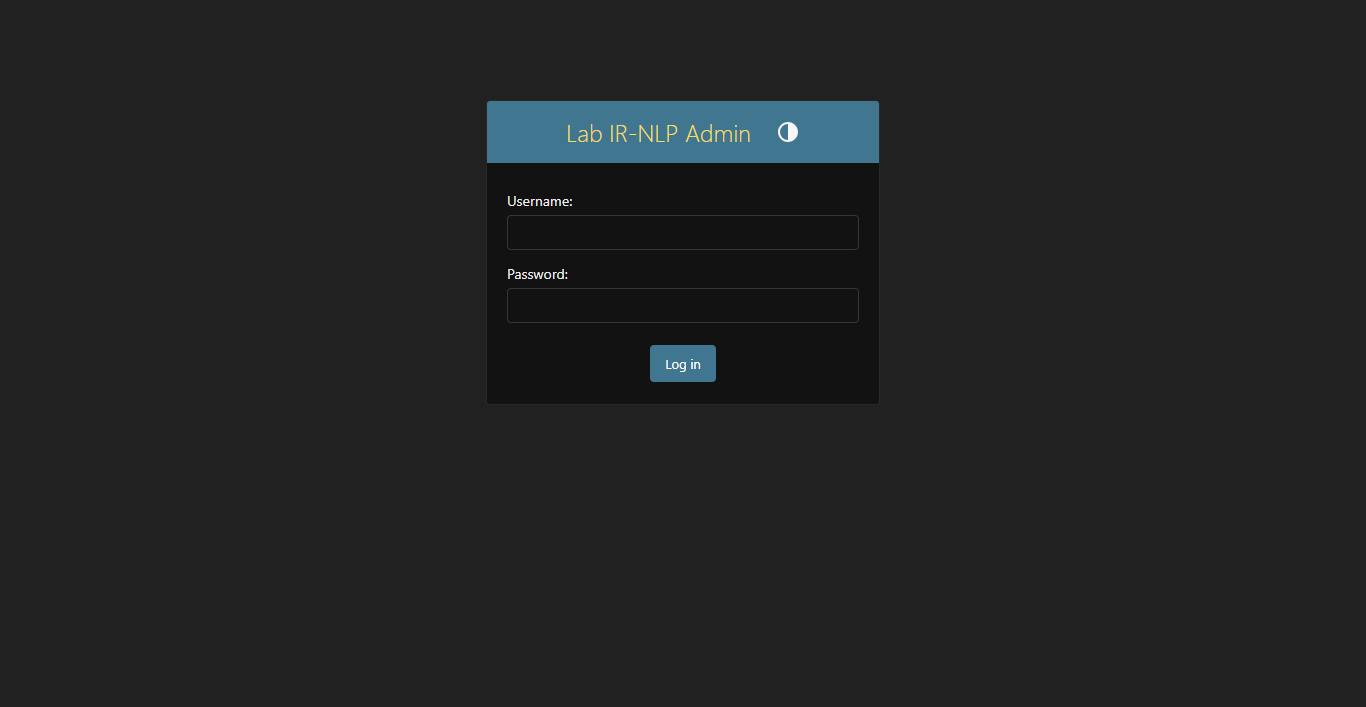
\includegraphics[width=8cm]{assets/pics/bab5_login.png}
    \caption{Halaman Login Admin}
    \label{fig:erd}
    \end{figure}
    \item Masukkan \textit{username} dan \textit{password} akun administrator yang telah dibuat sebelumnya.
    \item Setelah berhasil login, pengguna akan diarahkan ke halaman utama Admin Django yang berisi daftar model yang dapat dikelola.
\end{enumerate}

\begin{figure}[H]
    \centering
    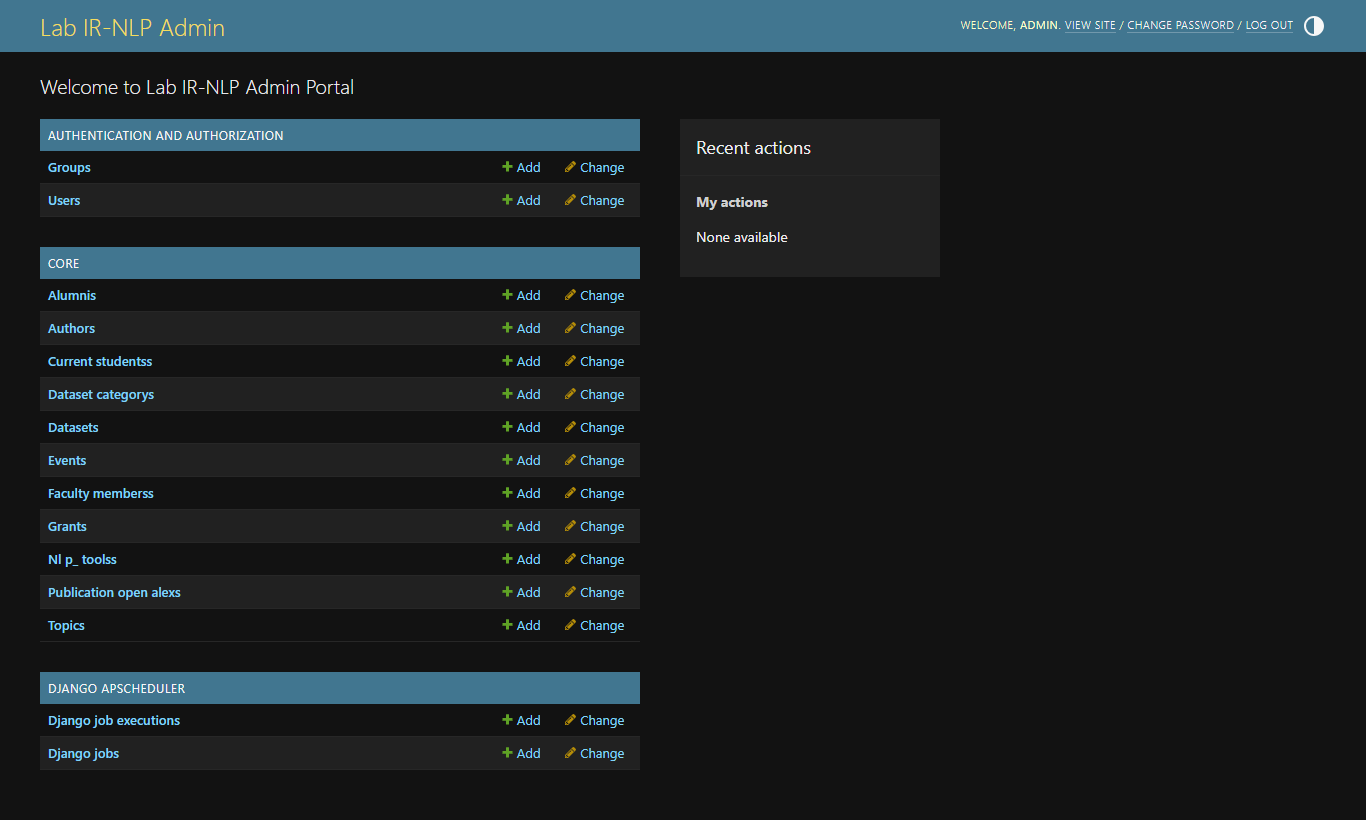
\includegraphics[width=8cm]{assets/pics/bab5_admin.png}
    \caption{Halaman Utama Admin}
    \label{fig:erd}
\end{figure}
Melalui halaman Admin Django, pengguna dapat melakukan berbagai aktivitas pengelolaan data, di antaranya:
\begin{itemize}
    \item \textbf{Menambah, mengedit, dan menghapus data publikasi} pada aplikasi \texttt{publications}.\\
    \begin{figure}[H]
    \centering
    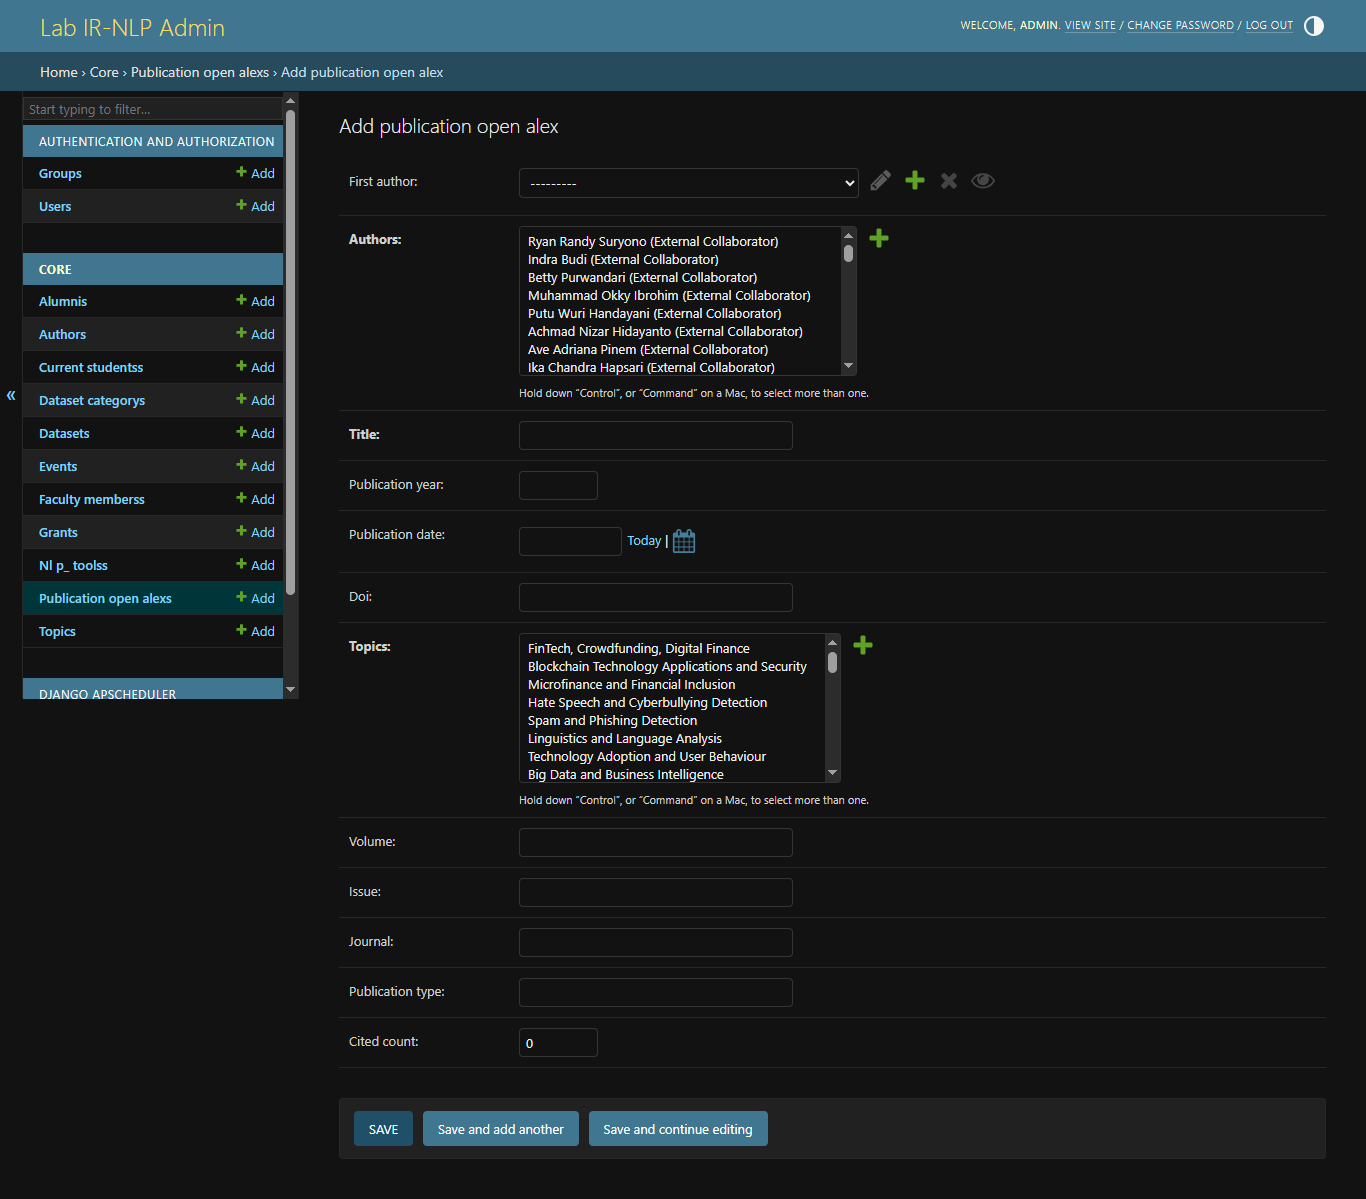
\includegraphics[width=8cm]{assets/pics/bab5_publications.png}
    \caption{Halaman Untuk menambahkan publikasi}
    \label{fig:erd}
\end{figure}
    Pengelolaan publikasi dilakukan melalui model \texttt{PublicationOpenAlex}. Untuk menambah data baru, pengguna dapat memilih menu \emph{Add Publication}, kemudian mengisi beberapa atribut berikut:
    
    \begin{itemize}
        \item \texttt{First Author}: penulis utama dari publikasi,
        \item \texttt{Authors}: dipilih dari daftar penulis yang tersedia,
        \item \texttt{Title}: judul publikasi,
        \item \texttt{Publication Year} dan \texttt{Publication Date},
        \item \texttt{DOI Link},
        \item \texttt{Topic},
        \item \texttt{Volume} dan \texttt{Issue},
        \item \texttt{Journal Name},
        \item \texttt{Publication Type} (misalnya: \textit{article}),
        \item \texttt{Citation Count}: jumlah sitasi.
    \end{itemize}
    Perlu dicatat bahwa data publikasi juga diatur melalui proses \textit{scraping}. Oleh karena itu, apabila terjadi perbedaan atau kesalahan data hasil \textit{scraping}, pengguna dapat melakukan pengeditan ulang dengan cara memilih salah satu objek publikasi, kemudian memperbarui atribut yang perlu diperbaiki.

    \item \textbf{Mengelola daftar anggota (members) atau pengguna yang terdaftar dalam sistem.}\\
    Terdapat tiga model utama untuk anggota, yaitu \texttt{Alumni}, \texttt{Faculty Members}, dan \texttt{Current Students}.

    \begin{itemize}
    \begin{figure}[H]
    \centering
    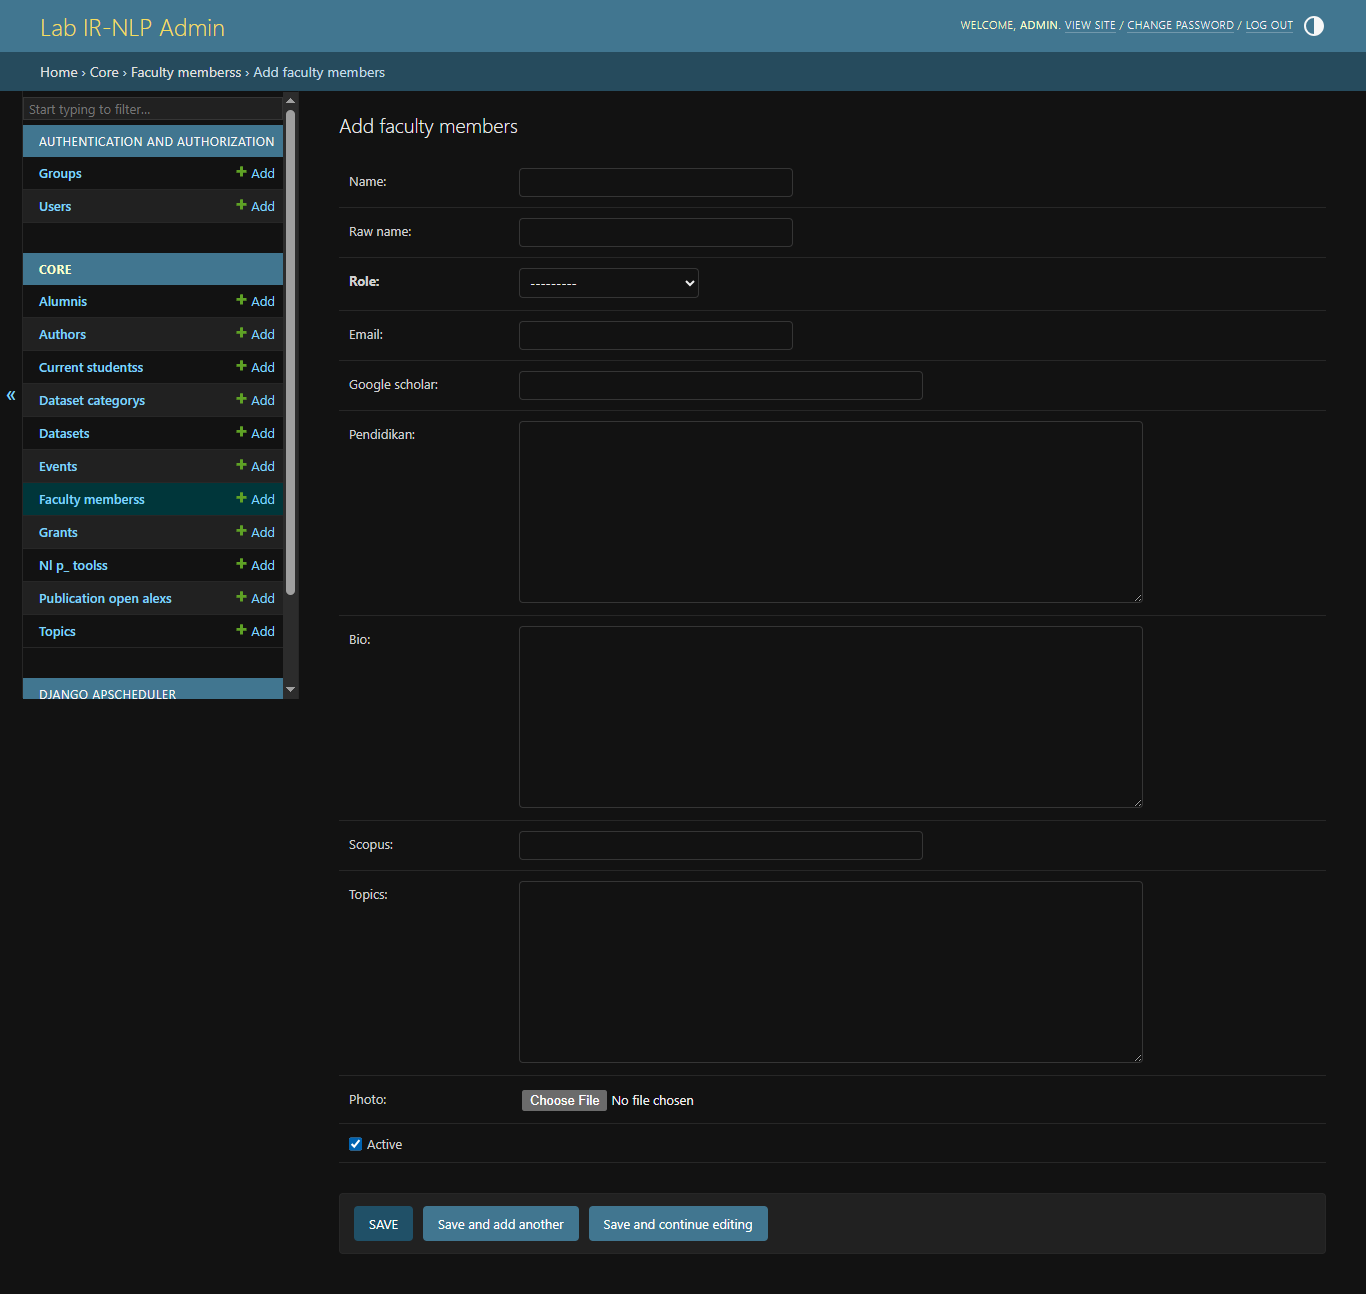
\includegraphics[width=8cm]{assets/pics/bab5_faculty_members.png}
    \caption{Halaman Untuk menambahkan Faculty Members}
    \label{fig:erd}
\end{figure}
        \item Untuk menambah atau mengedit \texttt{Faculty Members}, pengguna dapat memilih salah satu data yang tersedia atau menekan tombol \emph{Add Faculty Member}, kemudian mengisi:
        \begin{itemize}
            \item \texttt{Name}: nama yang ditampilkan pada halaman (termasuk gelar dan jabatan),
            \item \texttt{Raw Name}: nama asli tanpa gelar dan jabatan (digunakan untuk keperluan \textit{scraping}),
            \item \texttt{Role},
            \item \texttt{Email},
            \item \texttt{Google Scholar Link},
            \item \texttt{Education}: riwayat pendidikan yang dipisahkan dengan tanda koma, misalnya\\
            \textit{S1 Ilmu Komputer Universitas Indonesia, S2 Ilmu Komputer Universitas Indonesia},
            \item \texttt{Bio},
            \item \texttt{Scopus Link},
            \item \texttt{Research Topics},
            \item \texttt{Photo}.
        \end{itemize}
        Selain itu, terdapat tombol \texttt{Active} yang dapat dinonaktifkan apabila anggota tersebut sudah tidak aktif.
\begin{figure}[H]
    \centering
    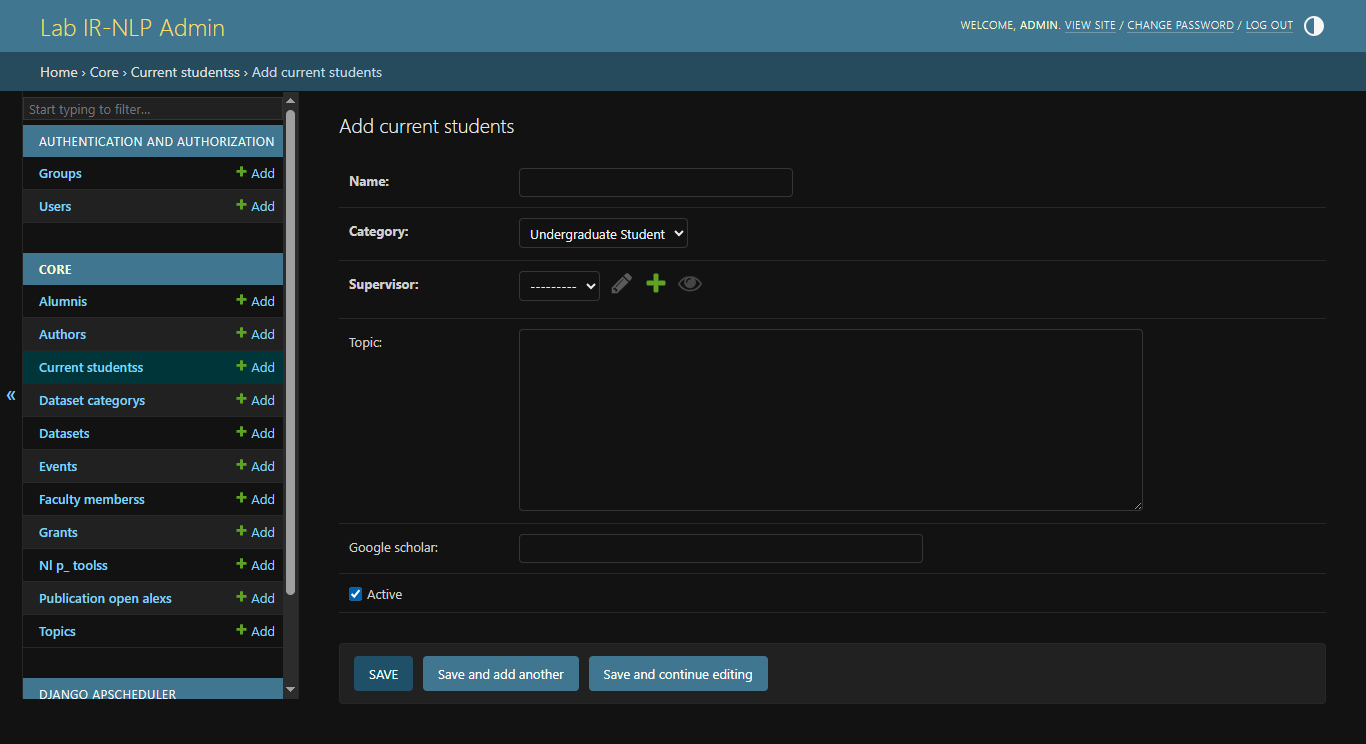
\includegraphics[width=8cm]{assets/pics/bab5_current_students.png}
    \caption{Halaman Menambahkan Mahasiswa}
    \label{fig:erd}
\end{figure}
        \item Untuk menambah atau mengedit \texttt{Current Students}, data yang harus diisi meliputi:
        \begin{itemize}
            \item \texttt{Name},
            \item \texttt{Category} (S1, S2, atau S3),
            \item \texttt{Supervisor} (1 orang dosen pembimbing),
            \item \texttt{Research Topic},
            \item \texttt{Google Scholar Link},
            \item \texttt{Active}.
        \end{itemize}
        Perlu dicatat bahwa terdapat logika otomatis pada sistem, di mana ketika tanggal kelulusan atau masa semester mahasiswa telah terlewati, maka statusnya akan secara otomatis berubah menjadi \textit{alumni}.
\begin{figure}[H]
    \centering
    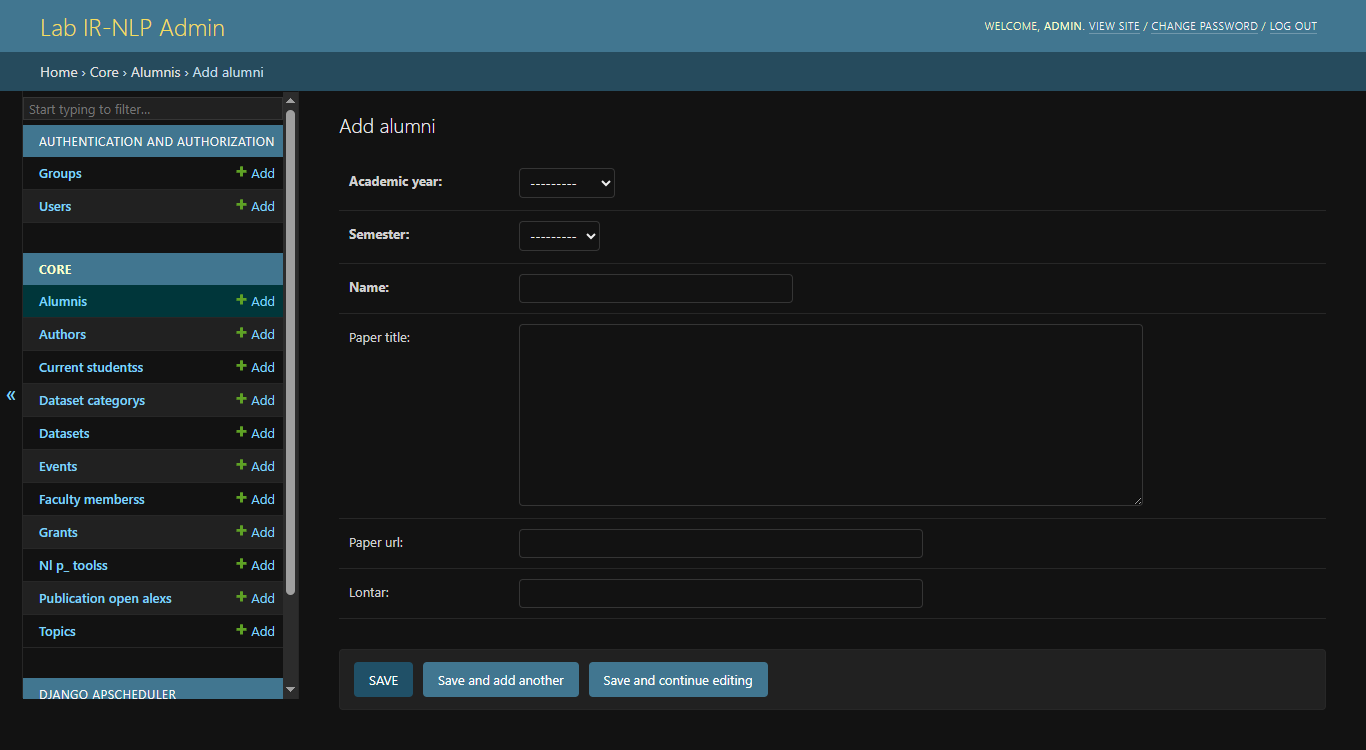
\includegraphics[width=8cm]{assets/pics/bab5_alumni.png}
    \caption{Halaman Menambahkan Alumni}
    \label{fig:erd}
\end{figure}
        \item Untuk menambah data \texttt{Alumni}, pengguna dapat mengisi:
        \begin{itemize}
            \item \texttt{Academic Year},
            \item \texttt{Semester},
            \item \texttt{Name},
            \item \texttt{Paper Title},
            \item \texttt{Paper Link},
            \item \texttt{Lontar Link}.
        \end{itemize}
    \end{itemize}
    
    \item \textbf{Menambah, memperbarui, dan menghapus data \textit{event}} pada aplikasi \texttt{events}.\\
    \begin{figure}[H]
    \centering
    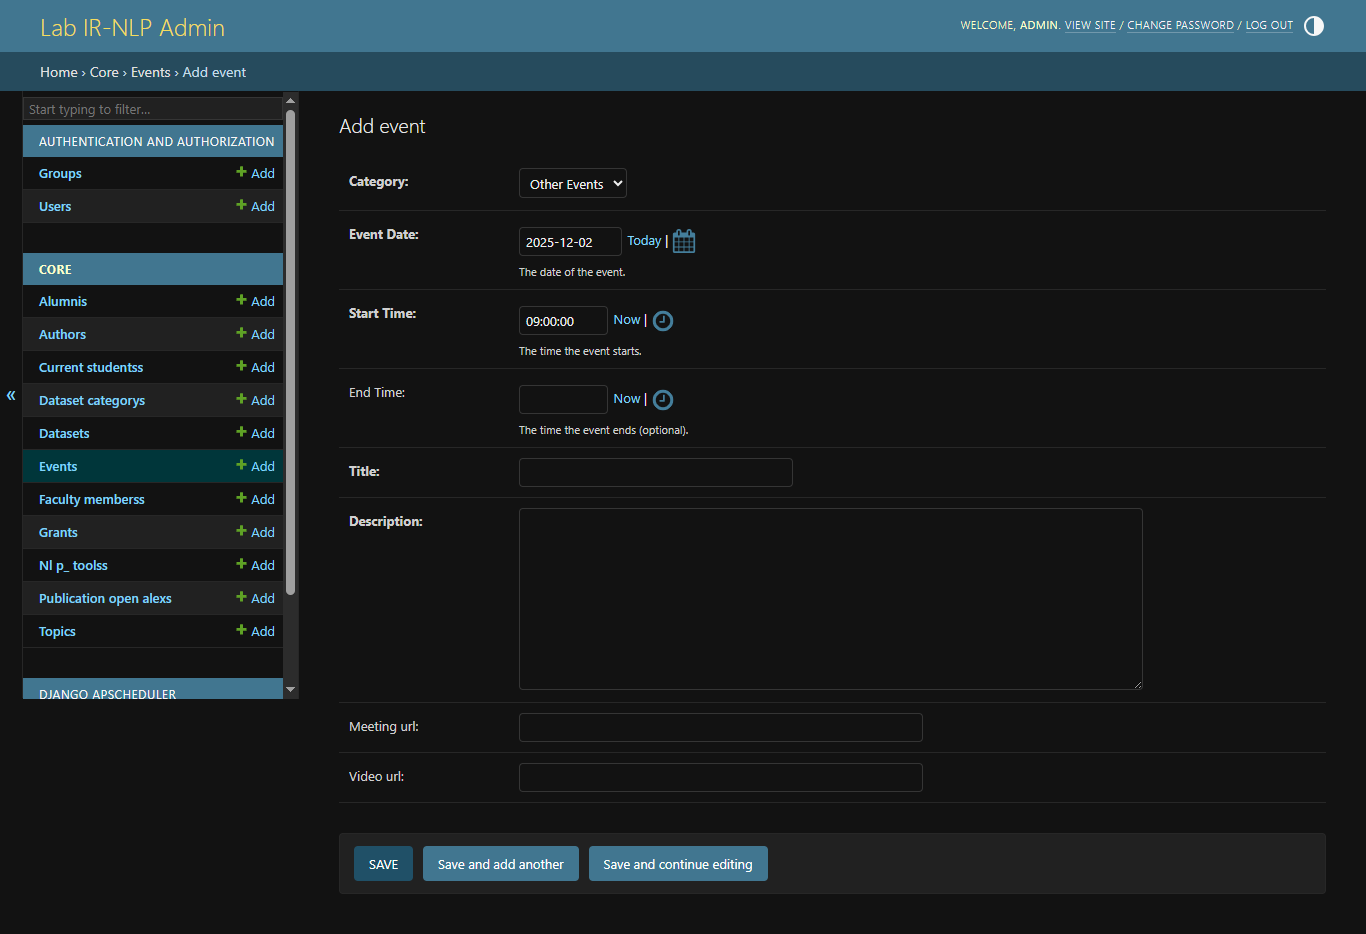
\includegraphics[width=8cm]{assets/pics/bab5_events.png}
    \caption{Halaman untuk Menambahkan Events}
    \label{fig:erd}
\end{figure}
Untuk menambahkan data \textit{event}, pengguna dapat menekan tombol \textit{Add Event} kemudian mengisi informasi berikut:
\begin{itemize}
    \item \texttt{Category}: kategori kegiatan,
    \item \texttt{Event Date}: tanggal pelaksanaan kegiatan,
    \item \texttt{Start Time}: waktu mulai,
    \item \texttt{End Time}: waktu selesai,
    \item \texttt{Title}: judul kegiatan,
    \item \texttt{Description}: deskripsi kegiatan,
    \item \texttt{Meeting URL}: tautan pertemuan daring,
    \item \texttt{Video URL}: tautan video atau rekaman kegiatan (jika tersedia).
\end{itemize}

\item \textbf{Menambah data \textit{Research Grant}.}\\
Penambahan data \textit{research grant} dapat dilakukan melalui dua cara, yaitu:
\begin{enumerate}
\begin{figure}[H]
    \centering
    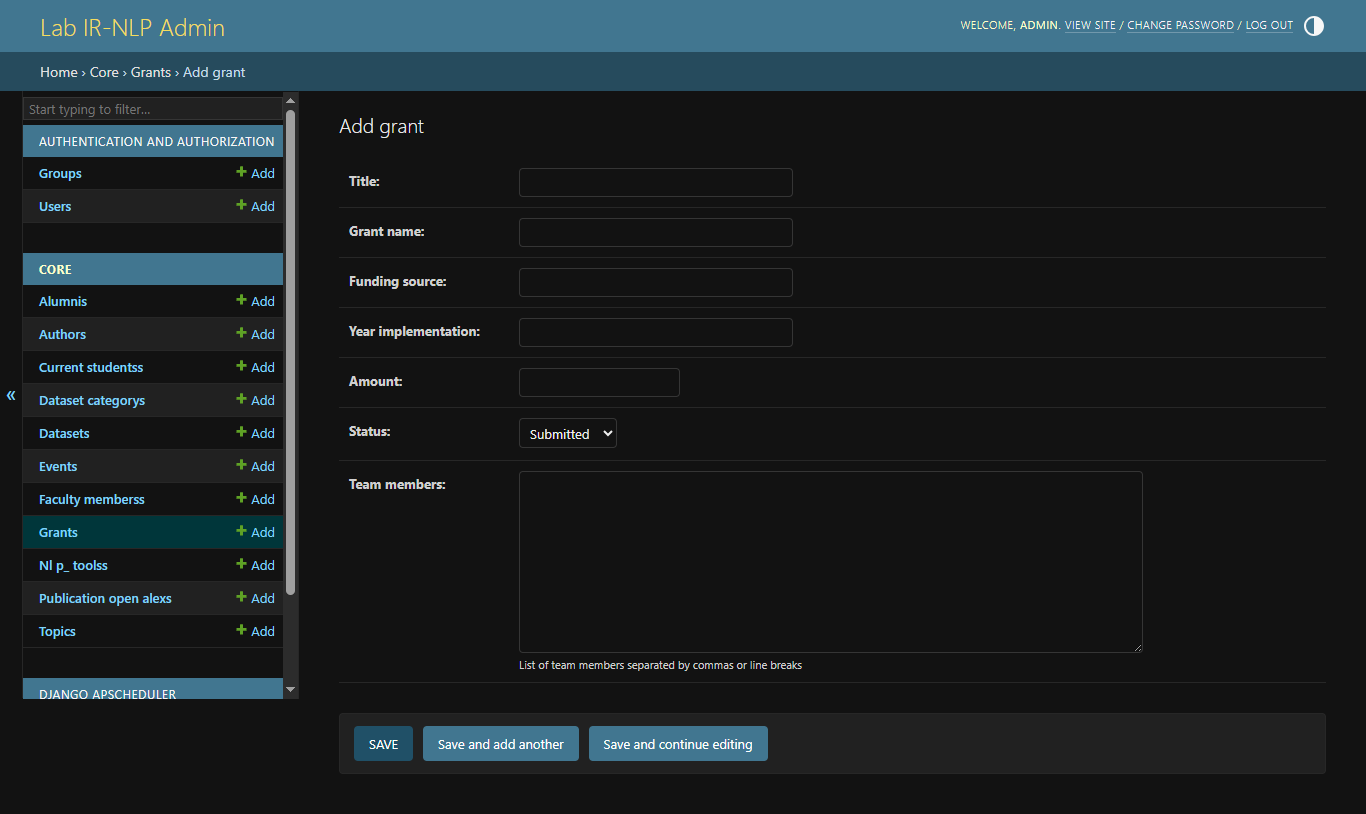
\includegraphics[width=8cm]{assets/pics/bab5_research_grant_sheets.png}
    \caption{Halaman Sheets untuk menambahkan Research Grant}
    \label{fig:erd}
\end{figure}
    \item Melalui Google Sheet yang telah disediakan, dengan mengisi data sesuai dengan kolom yang tersedia.
    \begin{figure}[H]
    \centering
    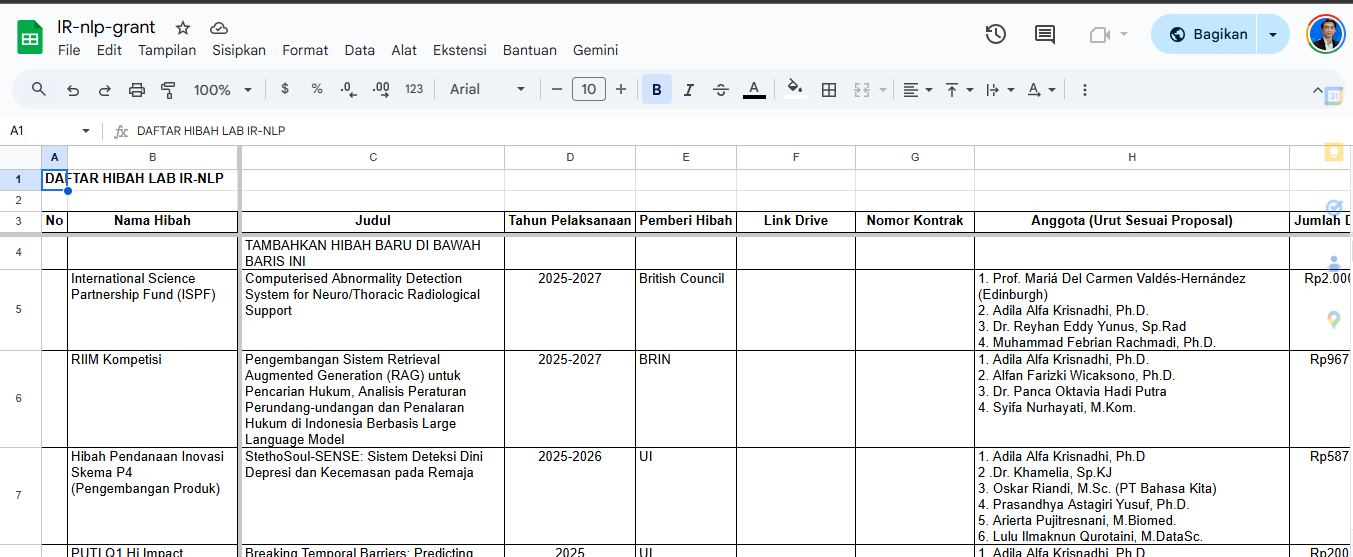
\includegraphics[width=8cm]{assets/pics/bab5_research_grant.png}
    \caption{Halaman untuk Menambahakn Research Grant}
    \label{fig:erd}
\end{figure}
    \item Melalui halaman Admin Django dengan memilih menu \textit{Add Grant} dan mengisi data yang diperlukan.
\end{enumerate}

\item \textbf{Menambah NLP Tools dari lab.}\\
Untuk menambahkan data \textit{NLP Tools}, pengguna dapat memilih menu \textit{Add NLP Tools}, kemudian mengisi informasi berikut:
\begin{figure}[H]
    \centering
    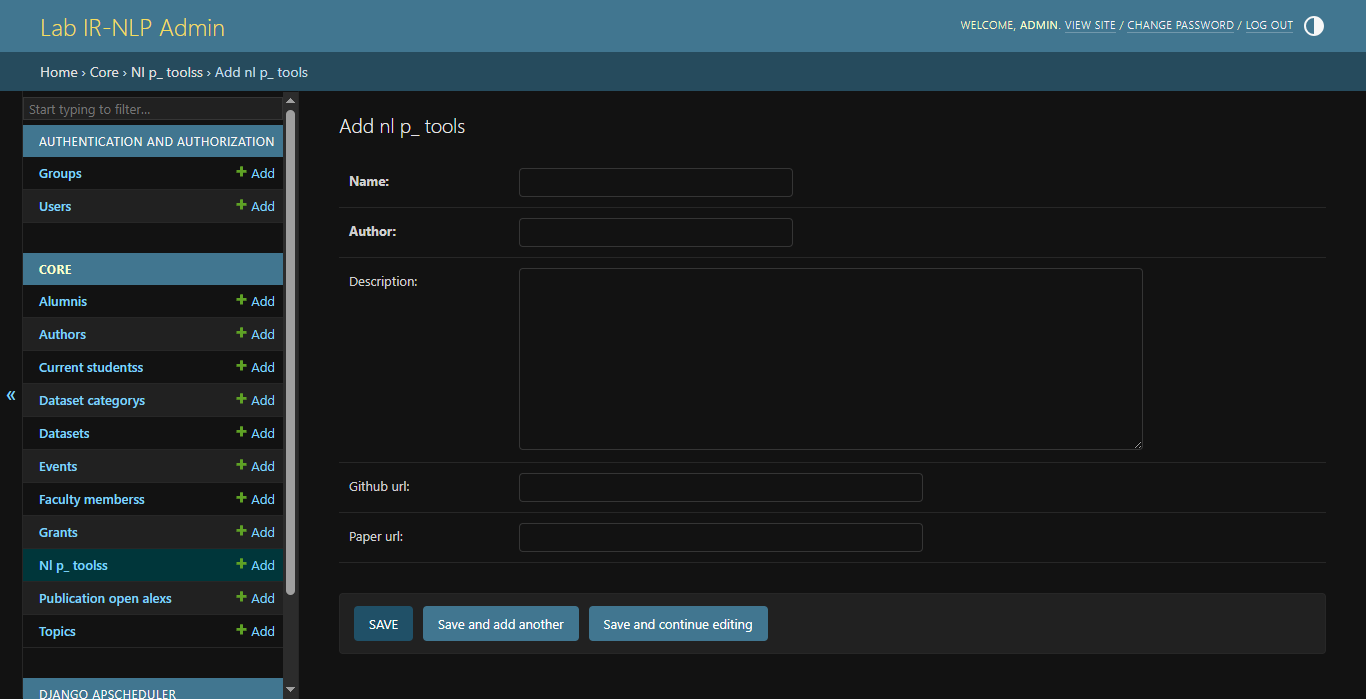
\includegraphics[width=8cm]{assets/pics/bab5_nlp_tools.png}
    \caption{Halaman untuk Menambahkan NLP Tools}
    \label{fig:erd}
\end{figure}
\begin{itemize}
    \item \texttt{Name}: nama tools,
    \item \texttt{Author}: pengembang atau pembuat tools,
    \item \texttt{Description}: deskripsi singkat tools,
    \item \texttt{GitHub URL}: tautan ke repositori GitHub,
    \item \texttt{Paper URL}: tautan ke publikasi ilmiah terkait.
\end{itemize}

\item \textbf{Menambah Dataset.}\\
Untuk menambahkan data dataset, pengguna dapat memilih menu \textit{Add Dataset}, kemudian mengisi:
\begin{figure}[H]
    \centering
    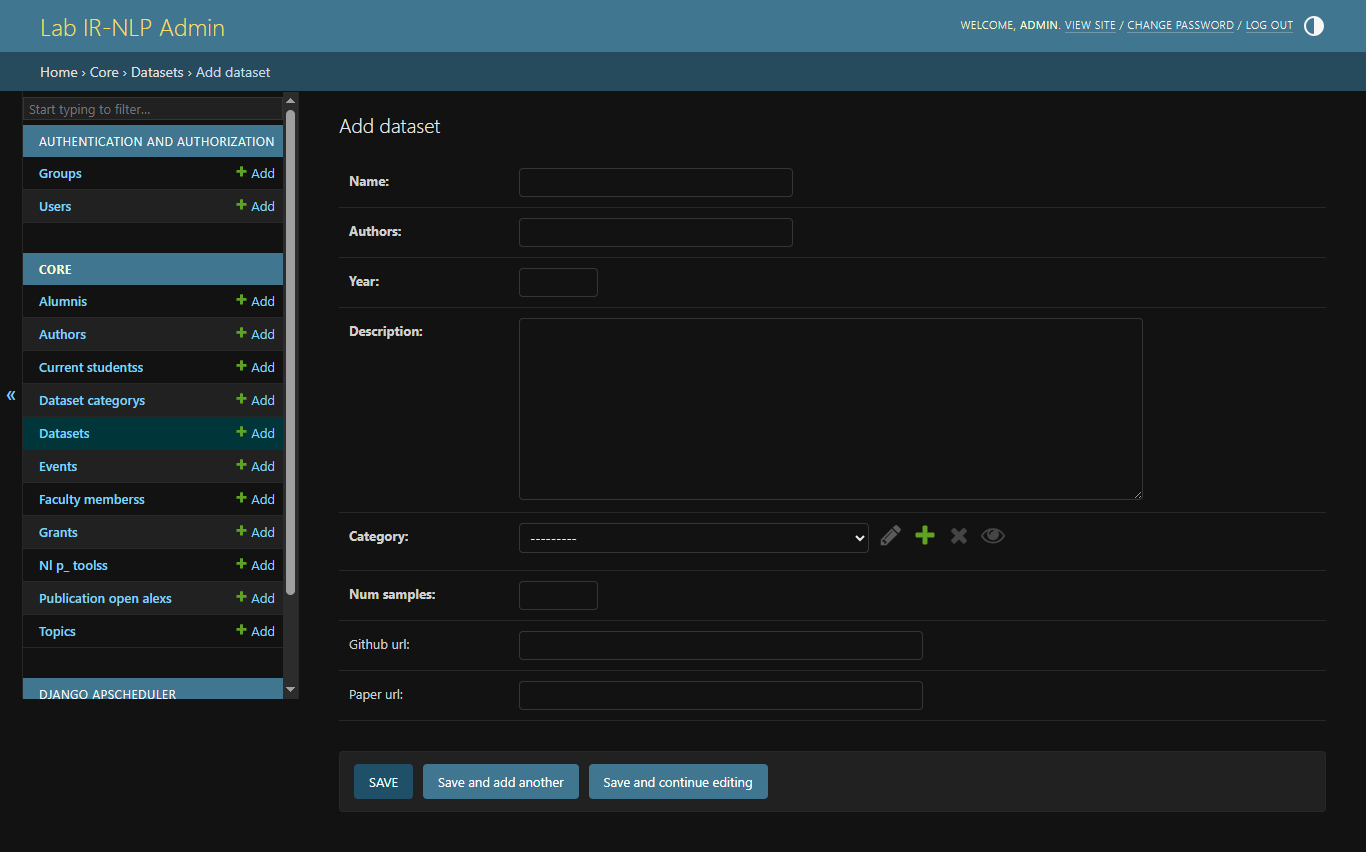
\includegraphics[width=8cm]{assets/pics/bab5_dataset.png}
    \caption{Halaman untuk Menambahkan Dataset}
    \label{fig:erd}
\end{figure}
\begin{itemize}
    \item \texttt{Dataset Name},
    \item \texttt{Authors},
    \item \texttt{Year},
    \item \texttt{Description},
    \item \texttt{Category},
    \item \texttt{Number of Samples},
    \item \texttt{GitHub URL},
    \item \texttt{Paper URL}.
\end{itemize}
\end{itemize}




